\section{Mandelbrot-Menge}
\label{julia:sec:mandelbrot}

Die Mandelbrot-Menge entsteht aus einer ähnlichen Überlegung wie die Julia- und Fatou-Mengen.
Auch hier werden Funktionen wiederholt auf Punkte angewendet, jedoch werden nur eine bestimmte Art von Funktionen sowie ein Punkt betrachtet.
Konkret werden quadratische Funktionen der Art
\begin{equation*}
    f_c(z) = z^2 + c,
\end{equation*}
sowie der Punkt $z = 0$ untersucht.

Auch hier erhält man eine Folge von Werten
\begin{equation*}
    z_0 \mapsto z_1 \mapsto z_2 \mapsto z_3 \mapsto \ldots\, ,
\end{equation*}
bzw.
\begin{equation*}
    0 \mapsto c \mapsto c^2 + c \mapsto c^4 + 2c^3 + c^2 + c \mapsto \ldots\, .
\end{equation*}

Nun lässt sich die \emph{Mandelbrot-Menge} als
\begin{equation*}
    M \coloneqq \left\{c \in \overline{\mathbb{C}}\:\mid\:f_c^n(0) \not\to \infty,\:\text{wenn}\:n \to \infty \right\}
\end{equation*}
definieren.
Das heisst, die Mandelbrot-Menge ist die Menge der Parameter $c$, für welche die Rekursion $z_{n+1}=z_{n}^{2} + c$ beschränkt bleibt, wenn man $z_0 = 0$ wählt.
Die Mandelbrot-Menge ist in der Abbildung \ref{julia:fig:mandelbrot_definition} dargestellt.
Wie diese Visualisierung entsteht, ist im Abschnitt \ref{julia:sec:visualisierung_mandel} beschrieben.
\begin{figure}
    \centering
    
\includegraphics[width=0.85\textwidth]{papers/julia/imgs/mandelbrot2.png}

    \caption{Die Mandelbrot-Menge}
    \label{julia:fig:mandelbrot_definition}
\end{figure}

Anhand obiger Definition wird der grundliegende Unterschied zwischen Julia- und Fatou-Mengen sowie der Mandelbrot-Menge klar.
Die Julia- und Fatou-Mengen sind im Zustandsraum der Dynamik, sie sind Teilmengen der $z$-Ebene.
Bei der Mandelbrot-Menge findet die Dynamik zwar auch in der $z$-Ebene statt, jedoch existiert die Mandelbrot-Menge im Parameterraum bzw. der $c$-Ebene.

Die Mandelbrot-Menge liegt vollständig innerhalb eines Kreises mit Radius $2$, jedoch gehört nicht der gesamte Kreisinhalt zur Mandelbrot-Menge.
Möchte man untersuchen, ob ein bestimmter Parameter $c_i$ zur Mandelbrot-Menge gehört, ist $|z_n| < 2$ für alle $n$ eine \emph{notwendige}, jedoch \emph{nicht hinreichende} Bedingung.

\subsection{Aufbau der Mandelbrot-Menge}
Betrachtet man die Mandelbrot-Menge \ref{julia:fig:mandelbrot_definition} erneut, so wird klar dass diese aus mehreren Komponenten besteht.
In Verbindung mit der Überlegung, welche die Julia-Mengen motivierte, lässt sich so ein interessanter Umstand beobachten.

So gibt es zum Beispiel die sogenannte Kardioide, welche die herzförmige und grösste Region der Mandelbrot-Menge ist.
Für jeden Parameter $c$ in der Kardioide, besitzt die zugehörige Funktion $f_c$ einen \emph{anziehenden} Fixpunkt $z_0$ (siehe Abschnitt \ref{julia:arten_periodische_punkte}), so dass
\begin{equation*}
    f_c(z_0) = z_0
\end{equation*}
gilt.
Anstatt als Fixpunkt könnte man diesen Punkt auch periodisch, mit einer Periode von $1$ nennen.

Angrenzend an die Kardioide liegen mehrere kreisförmige Knospen, die grösste davon befindet sich links der Kardioide.
Innerhalb dieser Knospe gilt für jeden Parameter $c$, dass die zugehörige Funktion $f_c$ einen \emph{anziehenden} periodischen Punkt $z_0$ besitzt, von dem eine Folge mit Periode $2$ ausgeht.
Für jede dieser Funktionen gibt es also einen Startwert, von dem sich eine Folge
\begin{equation*}
    z_0 \mapsto z_1 \mapsto z_0 \mapsto z_1 \ldots
\end{equation*}
entwickelt.
Aufgrund der Periodizität bezeichnet man diese Region als Periode-2 Knospe.

Die kleineren kreisförmigen Knospen verhalten sich ähnlich, es gibt
\begin{itemize}
    \item Periode-3 Knospen,
    \item Periode-4 Knospen,
    \item und so weiter.
\end{itemize}
Man kann also jede Region der Mandelbrot-Menge mit einer Periode bezeichnen.
Die Kardioide besitzt die Periode $1$, die grösste kreisförmige Knospe eine Periode von $2$ und so weiter.
Die unterschiedlichen Regionen sind also nicht nur dekorativ, sondern korrespondieren zu unterschiedlichen Arten von nicht-chaotischem, periodischem Verhalten.

\subsection{Verallgemeinerungen}
Die Mandelbrot-Menge lässt sich auf verschiedene Arten verallgemeinern.
In diesem Abschnitt werden einige davon beschrieben.

\subsubsection{Multibrot-Mengen}
Multibrot-Mengen entstehen, wenn man statt einer quadratischen Funktion, Polynome eines beliebigen Grades betrachtet
\begin{equation*}
    f_c(z) = z^d + c.
\end{equation*}
Beispiele davon sind in Abbildung \ref{julia:fig:multibrot_mengen} dargestellt.
Dies kann weiter verallgemeinert werden, indem negative und rationale Zahlen als Exponent $d$ erlaubt werden.
\begin{figure}
    \centering
    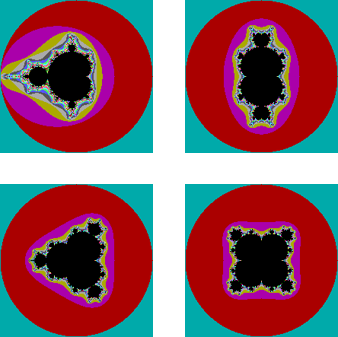
\includegraphics[width=\textwidth]{papers/julia/imgs/multibrot.png}

    \caption{Multibrot-Mengen für Polynome der Grade $2$, $3$, $4$ und $5$}
    \label{julia:fig:multibrot_mengen}
\end{figure}

\subsubsection{Höhere Dimensionen}
Statt den komplexen Zahlen kann auch mit \emph{Quaternionen} gearbeitet werden, diese sind die vierdimensionale Erweiterung der komplexen Zahlen.
Ein Quaternion wird als $q = a + bi + cj + dk$ notiert, mit $i^2 = j^2 = k^2 = ijk = -1$ und $i \ne j \ne k$.

Die vierdimensionale Mandelbrot-Menge kann dann in eine dreidimensionale Struktur projiziert werden, was jedoch relativ uninteressant ist, da es sich lediglich um die Mandelbrot-Menge, rotiert um die reelle Achse handelt \cite{julia:quaternionen}.

\subsubsection{Nicht-analytische Funktionen}
Statt holomorphen Funktionen können auch nicht-holomorphe bzw. nicht-analytische Funktionen verwendet werden.

Ein bekanntes Beispiel ist das Tricorn-Fraktal, dabei wird die Rekursion
\begin{equation*}
    z_{n+1} = \overline{z_n}^2 + c
\end{equation*}
verwendet.
Bevor $z_n$ quadriert wird, wird die komplexe Konjugation berechnet.

Ein weiteres Beispiel ist das Burning-Ship-Fraktal, welches durch die Rekursion
\begin{equation*}
    z_{n+1} = \left(|\text{Re}(z_n)| + i\,|\text{Im}(z_n)|\right)^2 + c
\end{equation*}
entsteht.
Anders als bei der Mandelbrot-Menge werden hier die Beträge des Real- und Imaginärteils berechnet, bevor quadriert wird.
